\documentclass[a4paper,fleqn]{article}

\usepackage{listings}
\usepackage{graphicx}
\usepackage{amsmath}
\usepackage{amssymb}
\usepackage{color}
\usepackage{array}
\usepackage{verbatim}
\usepackage{longtable}

\newcommand{\filename}[1]{
	\textsf{#1}
}
\newcommand{\code}[1]{
	\texttt{#1}
}
\newcommand{\external}[1]{
	\textbf{#1}
}

\newcommand{\thead}[1]{
	\textbf{#1}
}

%\usepackage[latin1]{inputenc}
%\usepackage[T1]{fontenc}

\lstset{language=C}

\begin{document}
\title{\Huge{EFSL}\\\Large{Embedded Filesystems Library - 0.3}}
\author{Lennart Yseboodt\\Michael De Nil}
\date{$\copyright$ 2005}
\maketitle

\newpage
\tableofcontents

\setlength{\parindent}{0pt}
\setlength{\parskip}{1ex plus 0.5ex minus 0.2ex}

\newpage
\section{Document Outdated!}
{\Huge{
This document is outdated and is in the progress of being renewed.\\
\newline\newline
If you are just starting with Efsl, we recommend you to start with the stable
0.2-branch. This version is currently not really usable, and is intended for people
working on the code.
}}
\newpage
\section{Preface}
\subsection{Project aims}
The EFSL project aims to create a library for filesystems, to be used on 
various embedded systems. Currently we support the Microsoft FAT filesystem 
family. It is our intention to create pure ANSI C code that compiles on 
anything that bears the name 'C compiler'. We don't make assumptions about 
endianness or how the memory alignment is arranged on your architecture.
\newline\newline
Adding code for your specific hardware is straightforward, just add code that 
fetches or writes a 512 byte sector, and the library will do the rest. 
Existing code can be used, writing your own code is only required when you 
have hardware for which no target exists.
\subsection{Project status}
Efsl currently supports FAT12, FAT16 and FAT32. Read and write has been tested 
and is stable. Efsl runs on PC (GNU/Linux, development environment), 
TMS C6000 DSP's from Texas instruments, and ATMega's from Atmel.
You can use this code with as little as 1 kilobyte RAM, however if you have 
more at your disposal, an infinite amount can be used as cache memory. 
The more memory you commit, the better the performance will be.
\subsection{License}
This project is released under the Lesser General Public license, which 
means that you may use the library and it's sourcecode for any purpose you want, 
that you may link with it and use it commercially, but that ANY change to the 
code must be released under the same license. We would appreciate if you would  send
us a patch when you add support for new hardware, but this is not obligatory, since it
falls under linking as far as the LGPL is concerned.

\newpage
\section{Getting started}
\subsection{On Linux (file) (0.2)}
	Debugging efsl on embedded devices is a rather hard job, because
you can't just printf debug strings or watch memory maps easily. 
Because of that, core development has been performed under the 
Linux operating system. Under Linux, efsl can be compiled as 
library and used as a userspace filesystem handler. On Unix-
style operating system (like Linux), all devices (usb stick, disc, \ldots)
can be seen as a file, and as such been opened by efsl.\newline
\newline
In the following section, we will explain how to get started using
efsl as userspace filesystem handler. However, please note that the main
focus for efsl is to support embedded systems, which usually don't even
have 1\% of the memory you have on a PC. Accessing files on a FAT-filesystem
with efsl will be much slower than when accessing these files with the Linux
FAT kernel modules.
\subsubsection{Download \& Compile}
Let's get started:
\begin{enumerate}
	\item{Get the latest release of efsl on http://www.sf.net/projects/efsl/ 
		and put it in your homedir}
	\item{Unpack the library (tar xvfj efsl-version.tar.bz2)}
	\item{Get inside the directory (cd $\sim$/efsl)}
	\item{Create a symlink from \filename{Makefile-LINUX} to \filename{Makefile} 
		(ln -s Makefile-LINUX Makefile)}
	\item{Copy \filename{conf/config-sample-linux.h} to \filename{conf/config.h}
		(cp conf/config-sample-linux.h conf/config.h)}
	\item{Compile the library (make lib)}
	\item{Find the compiled filesystem library (libefsl.a) in the current 
		directory}
\end{enumerate}
If you got any errors with the steps above, please check that that you have
the following packages installed: tar, gcc, libgcc, binutils \& make.
\subsubsection{Example}
Since efsl itself is only a library, it's not supposed to do anything
out of the box, than just compile. To get started, we'll show here a small
example program that opens a file on a disc/usb-stick/floppy that contains
a FAT-filesystem and prints it's content to stdout.\newline
\newline
First, create a new directory in which you put the compiled efsl-library
(\filename{libefsl.a}) and create a new file called \filename{linuxtest.c} containing:
\lstset{numbers=left, stepnumber=1, numberstyle=\small, numbersep=5pt, tabsize=4}
\begin{lstlisting}
	#include <stdio.h>
	#include <efs.h>
 
	int main(void)
	{
		EmbeddedFileSystem efs;
		EmbeddedFile file;
		unsigned short i,e;
		char buf[512];
	
		if(efs_init(&efs,"/dev/sda")!=0){
			printf("Could not open filesystem.\n");
			return(-1);
		}
	
		if(file_fopen(&file,&efs.myFs,"group",'r')!=0){
			printf("Could not open file.\n");
			return(-2);
		}

		while(e=file_read(&file,512,buf)){
			for(i=0;i<e;i++)
			printf("\%c",buf[i]);
		}
	
		return(0);
	}
\end{lstlisting}
$ $\newline
Some extra information on the code above:
\begin{itemize}
	\item{Line 1-2: The header files for stdio (used for printf) and efsl 
		are included. When using the basic efsl functions, \filename{efs.h} is
		the only header file of the efsl library that needs to be included.}
	\item{Line 6: The object efs is created, this object will contain 
		information about the hardware layer, the partition table and
		the disc.}
	\item{Line 7: The object file is created, this object will contain
		information about the file that we will open on the efs-object.}
	\item{Line 9: A buffer of 512 bytes is allocated. This buffer will
	 	be filled by fread with data.}
	\item{Line 11-14: Call of \code{efs\_init}, which will initialize the efs-object.
		To this function we pass:
		\begin{enumerate}
			\item{A pointer to the efs-object.}
			\item{A pointer to the file that contains the partition table /
				file system (in this example, we select a device as file).}
		\end{enumerate}
		If this function returns 0, it means that a valid fat partition is
		found on the device given. 
		If no valid fat-filesystem is found, or the file does not exist, the 
		function returns a negative value. In this example we then print an
		error message and quit.}
	\item{Line 16-19: Call of \code{file\_fopen()}, which will initialize the 
		file-object. To this function we pass:
		\begin{enumerate}
			\item{A pointer to the file-object.}
			\item{A pointer to the filesystem-object.} 
			\item{A pointer to the filename.}
			\item{A char containing the the mode (read, write, append).}
		\end{enumerate}
		If this function returns 0, it means the file has successfully been
		opened for reading / writing / appending.
		If the file could not be opened, a negative value is returned.
	}
	\item{Line 21-24: Call of \code{file\_read()}, which will read a given value of
		bytes (in this example 512) from a file and put it's content into
		the buffer passed (in this example called buf). This function returns
		the amount of bytes read, so the while-loop will be executed as long
		as there are bytes left in the file. The code inside the while-loop
		will print all characters in the buffer.}
\end{itemize}
\subsubsection{Testing}
So now let's test the program:
\begin{enumerate}
	\item{Compile the program 
		(gcc -I/home/user/efsl/inc/ -I/home/user/efsl/conf -o linuxtest 
		linuxtest.c -L./ -lefsl).}
	\item{Insert a usb-disc, floppy, mp3-stick, \ldots with a valid 
		fat-filesystem on it.}
	\item{Mount the device, copy the file /etc/group on it's root dir \& umount
		it.}
	\item{Check that you have permission to access the device
		(chown username /dev/sda*)}
	\item{Run the program (./linuxtest)}
\end{enumerate}












\newpage
\subsection{On AVR (SD-Card) (0.3)}
	This section describes how to implement Efsl on a AVR $\mu C$ connected to
an SD-Card (SPI). For getting efsl to compile, the avr-gcc compiler and 
avr-libc library are required. On Windows you should install WinAVR 
(http://winavr.sourceforge.net/), on Linux you can install the packages 
separately (see http://www.nongnu.org/avr-libc/user-manual/install\_tools.html
for a nice howto).
\subsubsection{Hardware}
First, you need set up a prototype in which you connect the CD, CMD, DAT0
\& CLK lines from the SD-Card to /CS, MOSI, MISO \& SCK from the Atmega.
\newline
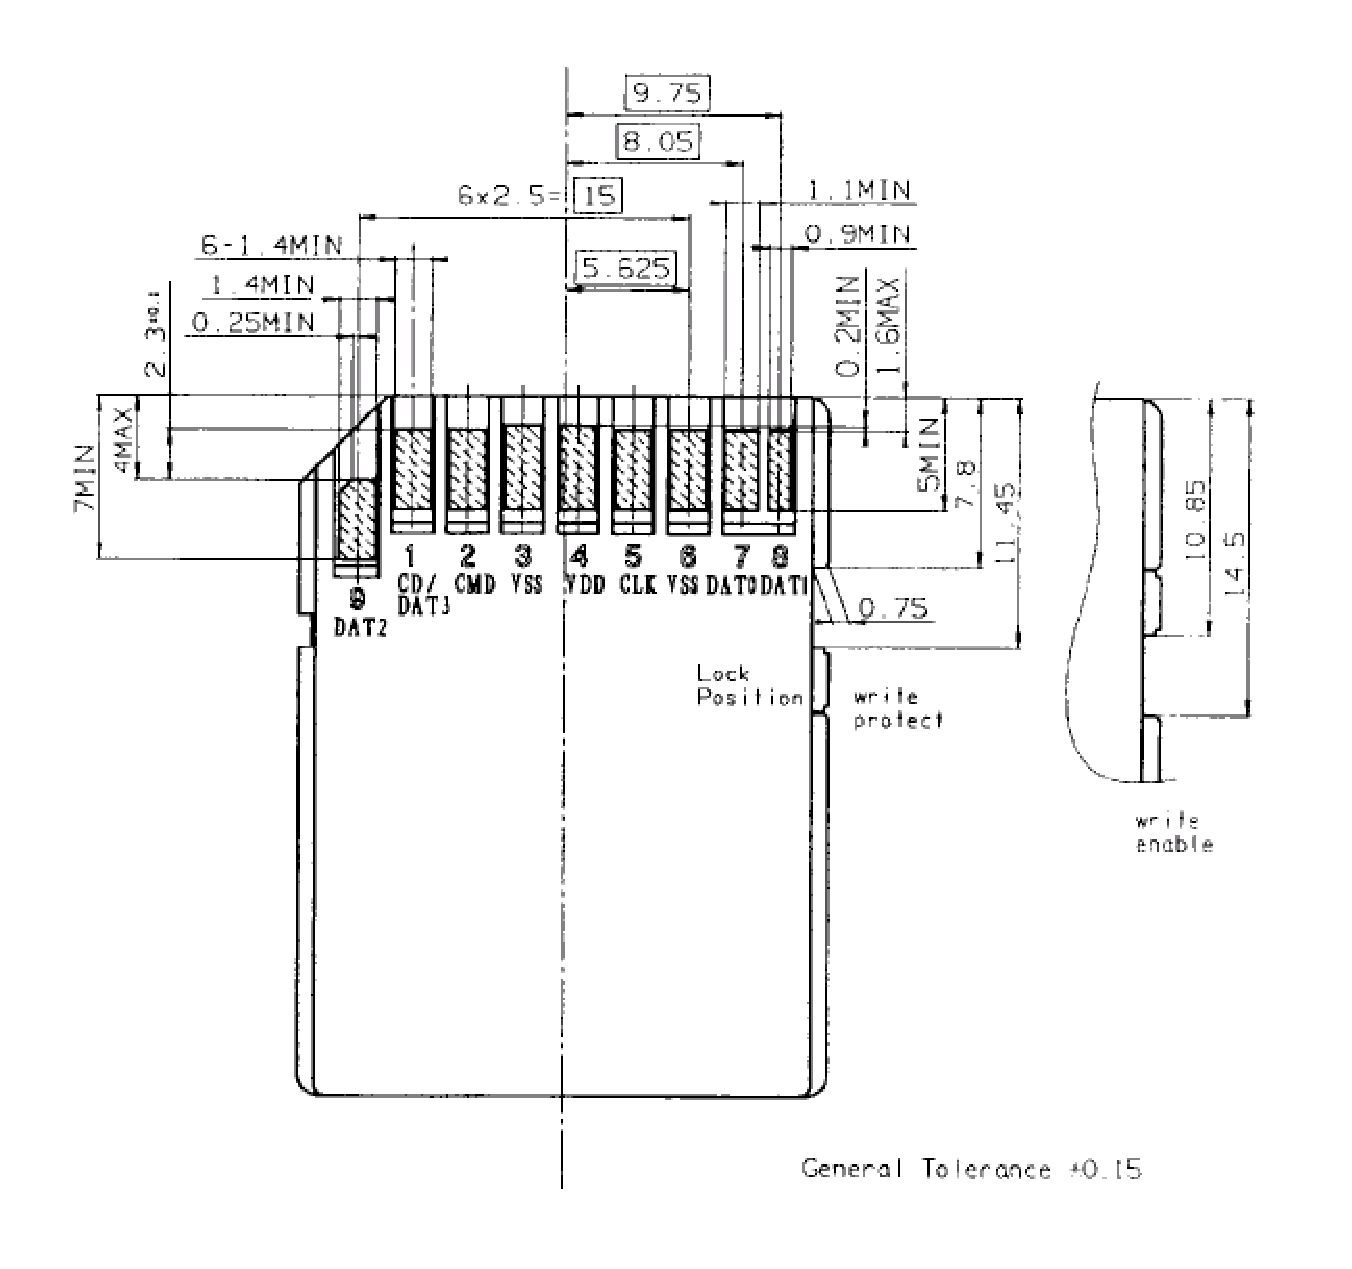
\includegraphics[scale=0.65]{pics/sdcard.eps}
\newline
%\parbox[c]{.4\textwidth}{\begin{center}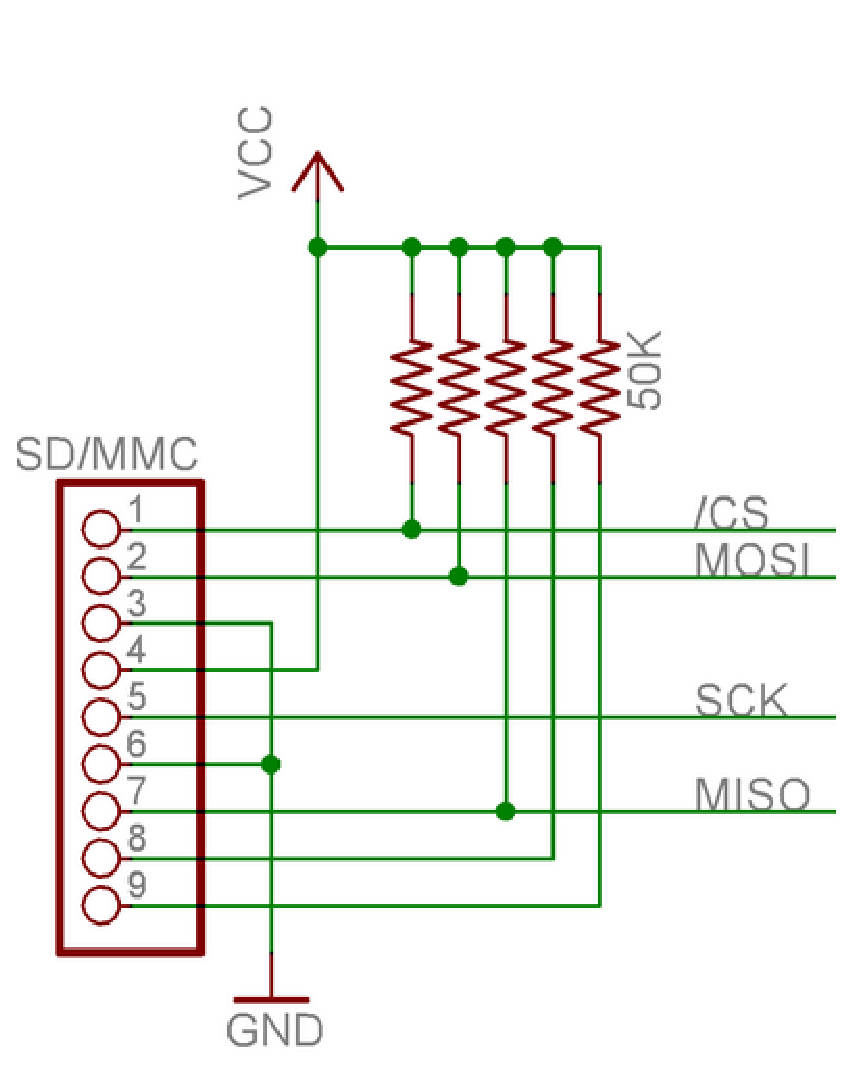
\includegraphics[width=.4\textwidth]{pics/sdconnection}\end{center}}
\parbox[c]{.5\textwidth}{
Connect the following lines on the SD-card:
\begin{itemize}
	\item{Pin 9 (DAT2) - NC\\(or pull-up to 3.3V)}
	\item{Pin 1 (CD) - Any pin on the Atmega128}
	\item{Pin 2 (CMD) - MOSI\\(pin 12 on the Atmega128)}
	\item{Pin 3 (Vss) - GND}
	\item{Pin 4 (Vdd) - +3.3V}
	\item{Pin 5 (CLK) - SCK\\(pin 11 on the Atmega128)}
	\item{Pin 6 (Vss) - GND}
	\item{Pin 7 (DAT0) - MISO\\(pin 12 on the Atmega128)}
	\item{Pin 8 (DAT1) - NC\\(or pull-up to 3.3V)}
\end{itemize}
}
\parbox[c]{.5\textwidth}{\begin{center}
	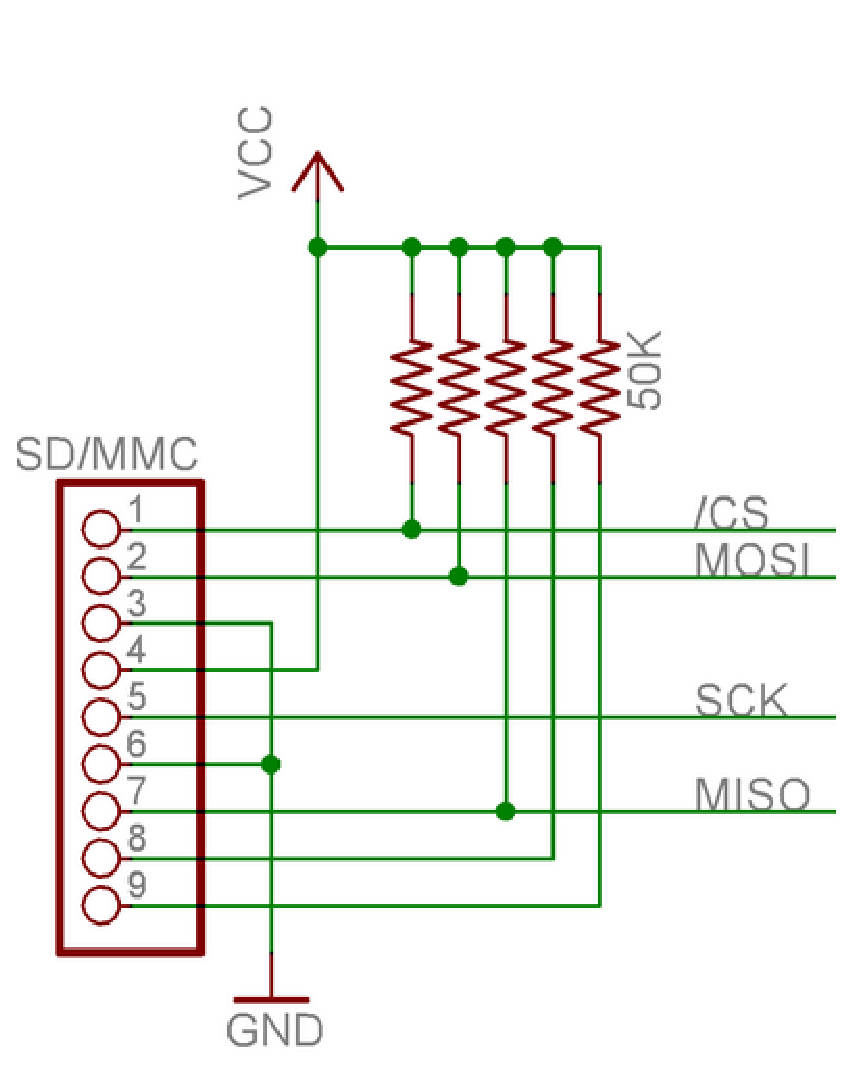
\includegraphics[width=.5\textwidth]{pics/sdconnection}
	\newline\newline
	Remark: this schematic includes pull-up's to 3.3V, which
	can be left off.
\end{center}}
\newline
Remark 1: Make sure that your $\mu C$ is running on 3,3V, so you don't
damage your SD-Card.\newline
\newline
Remark 2: CD is currently static set to PB0, but will become variable
in future releases.
\subsubsection{Download \& Compile}
Let's get started:
\begin{enumerate}
	\item{Get the latest release of efsl on http://www.sf.net/projects/efsl/}
	\item{Unpack the library (on Windows, you can use WinACE or WinRAR)}
	\item{Copy \filename{Makefile-AVR} to \filename{Makefile}}
	\item{Copy \filename{conf/config-sample-avr.h} to \filename{conf/config.h}}
	\item{Compile the library (\code{make lib})}
\end{enumerate}
Now you should have \filename{libefsl.a} in the efsl directory.
\subsubsection{Example}
Since Efsl itself is only a library, it's not supposed to do anything out of 
the box, than just compile. To get started, we'll show here a small example
program that opens an existing file and writes the content to a new file.
\newline\newline
First, create a new directory in which you put the compiled efsl-library 
(\filename{libefsl.a}) and create a new file called \filename{avrtest.c} containing:
\lstset{numbers=left, stepnumber=1, numberstyle=\small, numbersep=5pt, tabsize=4}
\begin{lstlisting}
	#include <efs.h>

	void hang(void);

	void main(void)
	{
		EmbeddedFileSystem efs;
		EmbeddedFile file_r, file_w;
		unsigned short i,e;
		char buf[512];

		if(efs_init(&efs,0)!=0){
			hang();
		}

		if(file_fopen(&file_r,&efs.myFs,"orig.txt",'r')!=0){
			hang();
		}

		if(file_fopen(&file_w,&efs.myFs,"copy.txt",'w')!=0){
			hang();
		}

		while(e=file_read(&file_r,512,buf)){
			file_write(&file_w,e,buf);
		}

		file_fclose(&file_r);
		file_fclose(&file_w);

		fs_umount(&efs.myFs);

		hang();
	}

	void hang(void)
	{
		while((1))
			_NOP();
	}
\end{lstlisting}
$ $\newline
Some extra information on the code above:
\begin{itemize}
	\item{Line 1: The header file for efsl is included here. When using the
		basic efsl functions, \filename{efs.h} is the only header file on the 
		efsl library that needs to be included.}
	\item{Line 7: The object efs is created, this object will contain
		information about the hardware layer, the partition table and
		the disc.}
	\item{Line 8: The objects \code{file\_r} and \code{file\_w} are created, these objects 
		will contain information about the files that we will open on the 
		efs-object.}
	\item{Line 9: A buffer of 512 bytes is allocated. This buffer will be
		used for reading and writing blocks of data.}
	\item{Line 12: Call of \code{efs\_init()}, which will initialize the efs-object.
		To this function we pass:
		\begin{enumerate}
			\item{A pointer to the efs-object.}
			\item{A pointer to the file that contains the partition table /
				file system (in this example, we select a device as file).}
		\end{enumerate}
		If this function returns 0, it means that a valid fat partition is
		found on the SD-card connected.
		If no valid fat-filesystem is found, or the file does not exist, the
		function returns a negative value. In this example we then go to an
		infinite loop to prevent the program to continue.}
	\item{Line 16 \& 20: Call of \code{file\_fopen()}, which will initialize the
		file-objects. To this function we pass:
		\begin{enumerate}
			\item{A pointer to the file-object.}
			\item{A pointer to the filesystem-object.}
			\item{A pointer to the filename.}
			\item{A char containing the the mode (read, write, append).}
		\end{enumerate}
		If this function returns 0, it means the file has successfully been
		opened for reading / writing / appending.
	 	If the file could not be opened (because for example a file already 
		exists), a negative value is returned.}
	\item{Line 24: Call of \code{file\_read()}, which will read a given value of
		bytes (in this example 512) from a file and put it's content into
		the buffer passed (in this example called buf). This function returns
		the amount of bytes read, so the while-loop will be executed as long
		as there are bytes left in the file.}
	\item{Line 25: Call of \code{file\_write()}, which will write a given value
		of bytes (in this example, the amount of bytes that was read
		by \code{file\_read()}) from the buffer passed to a file. This function returns
		the amount of bytes written.}
	\item{Line 28 \& 29: Call of \code{file\_fclose()}, which will close the
		file-objects.}
	\item{Line 31: Call of \code{fs\_umount()}, which will write all buffers to
		the the SD-card.}
\end{itemize}
\subsubsection{Testing}
So now let's test the program:
\begin{enumerate}
	\item
	{
		Make sure that your directory contains both the example from above
		called \filename{avrtest.c} and the library \filename{libefsl.a}.
	}
	\item
	{	Compile the program:
		\begin{itemize}
			\item{On Linux (with avr-gcc): avr-gcc -I/home/user/efsl/inc/ 
				-I/home/user/efsl/conf -ffreestanding -mmcu=atmega128 -Os -o 
				avrtest.o avrtest.c -L./ -lefsl}
			\item{On Windows (with WinAVR): avr-gcc 
				-Ic:$\backslash$efsl$\backslash$inc
				-Ic:$\backslash$efsl$\backslash$conf 
				-ffreestanding -mmcu=atmega128 -Os -o
				avrtest.o avrtest.c -L.$\backslash$ -lefsl}
		\end{itemize}
	}
	\item{Generate a hexfile 
		(avr-objcopy -j .text -j .data -O ihex avrtest.o avrtest.hex)}
	\item{Connect an SD-card to your Atmega128 with a file called 
		\filename{orig.txt} on it.}
	\item
	{
		Flash the hex file into your $\mu C$.
		\begin{itemize}
			\item{On Linux: avrdude -P /dev/ttyUSB0 -c stk500 -p m128 -Uflash:w:avrtest.hex}
			\item{On Windows: use Atmel AVR-Studio}
		\end{itemize}
	}
	\item{Reset your $\mu C$ and wait some time (depending on how big
		the file \filename{orig.txt} is).}
	\item{Disconnect the SD-card, so you can put it in your card reader
		and find out if the file \filename{orig.txt} is copied to 
		\filename{copy.txt}.}
\end{enumerate}

\newpage
\subsection{On DSP (SD-Card) (0.2)}
	This section will tell you everything you need to know to start using the
embedded filesystems library on a TMS Digital Signal Processor from Texas Instruments.
The only thing that is required is that you have a McBSP port available, and that your DSP
support CLOCKSTOP mode, which is required to connect a SPI compatible device.

There are special DSP's from TI which have a special MMC/SD card controller, if you want to
use this special interface you will have to create a hardware endpoint for it. This section only
describes connecting an SD card to a normal McBSP port, since every TI DSP has at least one of them.

\subsubsection{Hardware}
Connecting the SD card to the McBSP is straightforward, you will have to make 4 data related
connections, Vcc and ground, resulting in a 6 wire interface.\\
\begin{tabular}{|l|l|l|l|l|}
	\hline
	\multicolumn{3}{|c|}{SD Card Interface}&\multicolumn{2}{|c|}{McBSP Interface}\\
	\hline
	1 & CS & Chip select & FSX & Frame Sync Transmit \\
	2 & MOSI & Master out Slave In & DX & Data transmit \\
	3 & GND & Supply Ground &&\\
	4 & Vcc & Supply voltage (3.3 Volt) &&\\
	5 & Clk & Clock & CLKX & Clock Transmit\\
	6 & GND & Supply ground &&\\
	7 & MISO & Master in Slave out & DR & Data receive \\
	8 & NC & Not connected &&\\
	9 & NC & Not connected &&\\
	\hline
\end{tabular}\\
You can optionally pull the DataIn and DataOut lines up to Vcc with a $10k\Omega$ resistor, but
we found that this was not required for operation.\\
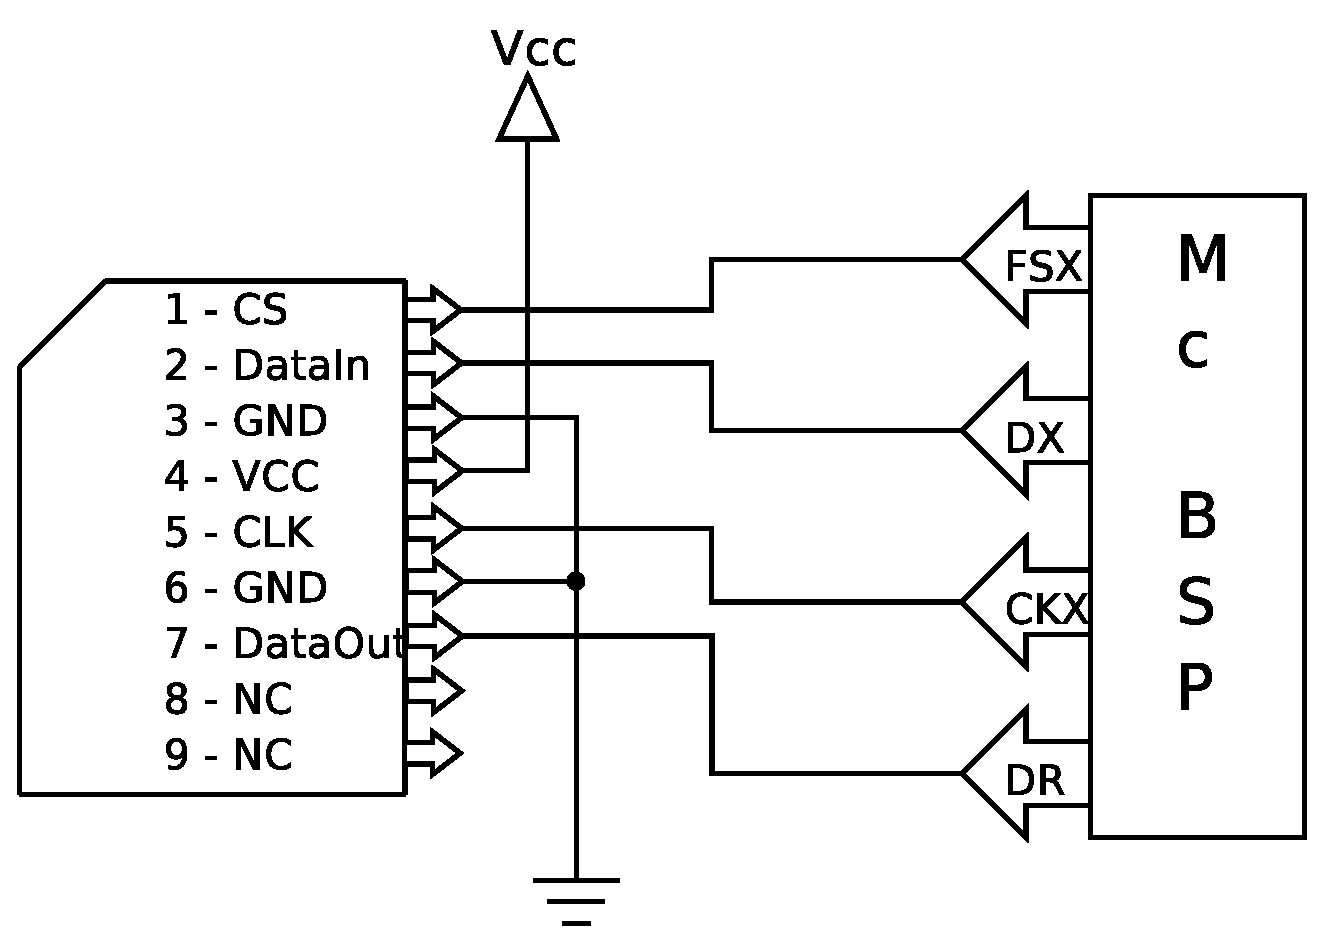
\includegraphics[scale=0.4]{schematics/sdcard.eps}\\
The frame sync from the McBSP port is used to select the card whenever a databyte has to be transferred, it is connected to the chip select of the SD card. The DX and DR pins are connected to the SDcard's DataIn and DataOut lines respectively. Finally the McBSP will have to generate a clock for
the SDcard so that it can perform operations, this is accomplished by connecting the clock transmit
line of the McBSP port to the CLK pin of the SDCard.

\subsubsection{McBSP configuration}
\begin{longtable}{|p{0.13\textwidth}|p{0.1\textwidth}|p{0.06\textwidth}|p{0.75\textwidth}|}
	
	\hline
	\multicolumn{4}{|c|}{
		\textbf{McBSP Register Explanations}
	} \\
	\hline
	\hline
	\endfirsthead
	
	\hline
	\multicolumn{4}{|c|}{\textbf{mcbsp registers (continued)}} \\
	\hline
	\endhead
	\hline
	\endfoot
	
	\hline 
	\endlastfoot

 	\multicolumn{3}{|c|}{SPCR}&
 	\multicolumn{1}{c|}{Serial Port Control Register}\\
 	\hline
 	Name & Bit & Value &\multicolumn{1}{c|}{Value \code{(0x00001800 | 0x00410001)}}\\
 	\hline
	RRST&\code{0}&\code{1b} & The serial port receiver is enabled \\
	XRST&\code{16}&\code{1b} & The serial port transmitter is enabled \\
	CLKSTP&\code{12:11}&\code{11b} & Clock starts on falling edge without delay(see CLKXM) \\
	GRST&\code{22}&\code{1b} & Sample rate generator is pulled out of reset \\
	\hline

 	\multicolumn{3}{|c|}{PCR}&
 	\multicolumn{1}{c|}{Pin Control Register}\\
 	\hline
 	Name &Bit & Value &\multicolumn{1}{c|}{Value \code{0x00000A0C}}\\
 	\hline
	CLKXP&\code{1} &\code{0b} & Transmit data on the rising edge ofthe clock\\
	FSXP&\code{3} &\code{1b} & Frame Sync (Chip select on SD card) is active low\\
	CLKXM&\code{9} &\code{1b} & McBSP is a master in SPI mode and generates the clock based on
	                            the sample rate generator\\
	FSXM&\code{10} &\code{1b} & Frame sync is determined by tge sample rate generator\\
	\hline

 	\multicolumn{3}{|c|}{RCR/XCR}&
 	\multicolumn{1}{c|}{Receive/Transmit Control Register}\\
 	\hline
 	Name &Bit & Value &\multicolumn{1}{c|}{Value \code{0x00010000}}\\
 	\hline
	RWDLEN&\code{7:5} &\code{000b} & Receive element is 8 bits (1byte) large\\
	XDATDLY&\code{17:16} &\code{01b} & 1 bit data delay (after frame sync)\\
	\hline

 	\multicolumn{3}{|c|}{SRGR}&
 	\multicolumn{1}{c|}{Sample Rate Genrator}\\
 	\hline
 	Name &Bit & Value &\multicolumn{1}{c|}{Value \code{0x20000002}}\\
 	\hline
	CLKSM&\code{29} &\code{1b} & The sample rate generator clock is derived from the internal clock\\
	FSGM&\code{28} &\code{0b} & The transmit frame sync signal is generated on every DXR to XSR copy\\
	CLKGDV&\code{7:0}&\code{0x02h} & The clock divider\\
	\hline

\end{longtable}


\newpage
\section{Configuring EFSL (0.2)}
	In this section we're going to talk about the configuration file (\filename{config.h}),
that defines the behavior of the library. In the configuration files there are many
settings, most of which default to safe or 'standard' compliant settings.

For every platform we try to deliver a sample configuration, with setting tweaked for
that architecture. This documentation only refers to the general elements which are
tied to the library rather that the target hardware.

\subsection{Hardware target}
Here you will define what kind of hardware you will be using. Please refer to
section \ref{hwdriver} to learn how to write a hardware endpoint.
Here you must \code{\#define} the name of your hardware endpoint.
The following list contains the endpoints that the library ships with.\\
\begin{tabular}{|l|p{8cm}|}
	\hline
	\code{HW\_ENDPOINT\_LINUX}& This endpoint uses a regular file as
	a "disc" containing a filesystem. This is a great endpoint for
	testing and debugging. All development is done using this emulation.\\
	\code{HW\_ENDPOINT\_ATMEGA128\_SD}& This endpoint is for the Atmel ATMega 128
	with an SD card attached to the SPI pins of the device. Several settings
	that are specific for this endpoint can be found in the AVR sample 
	configuration. A Makefile is also provided for compiling the EFSL library
	using avr-gcc.\\
	\code{HW\_ENDPOINT\_DSP\_TI6713\_SD}& This endpoint is for a TI DSP, it should
	work with any McBSP port, due to the infinite amount of options, you should
	refer to the source code of this endpoint for fine tuning, or selecting what
	port to use (defaults to McBSP0).\\
	\hline
\end{tabular}

\subsection{Memory configuration}
This section only has one option, called \code{BYTE\_ALIGNMENT}. If you define
this keyword the library will assume that your CPU is capable of accessing the
memory in any way it sees fit. This is the case on AVR, because they are 8 bit
processors, and it is also the case on Intel x86 hardware. Both architectures can
read and write words, or double words on any location in memory, be it word aligned
or not.

However, some CPU's, are not capable of doing this, and require that all double words
are aligned on a double word boundary, and all word are aligned on a word boundary.
This causes problems with some of the casts that are performed in EFSL. If you have such
a CPU, then you must comment this option out. The effect is that special functions
will be used to copy or cast memory. These functions work around the problem by
using memCpy, or manually copying elements of the structs that are normally cast when
\code{BYTE\_ALIGNMENT} is defined.

If you have an 8 bit architecture, or are running on PC, there is no need to turn this
off. If you do, the library will work fine, and maybe even without slowdown.
On architectures that do have the alignment problem, you should turn this flag off.
Failure to do so will result in undefined behavior.

\subsection{Cache configuration}
This section is dedicated to configuring the cache memory for the library. Caching
is performed by the IOMan object, see section \ref{ioman}.
\subsubsection*{IOMAN\_NUMBUFFER}
This number determines how much memory will be used for caching. Since this
is sector based one \code{IOMAN\_NUMBUFFER} equals to 512 byes of memory, plus
a small overhead in settings (approximately 8 bytes). This number is also affected
by \code{IOMAN\_NUMITERATIONS}. 

You should carefully consider how much memory you will dedicate to caching. A too
low number will cause excessive data transfer to and from the disc, where a too high
number will simply be a waste of memory.

A good rule of thumb is to use 1 buffer per filesystem you create, and 2 buffers
per file you want to use simultaneously. So for a simple application with
one filesystem, and one file operation, 2 or 3 buffers will be fine. If you have memory
to spare, you can use 6 buffers. Using more buffers will have a minimal effect on
performance.

If you want to seek and rewrite portions of a file, add an extra buffer for that file.
Using the list function or creating directories will be disc intensive, try to smoothen
it by using an extra 3 buffer for either operation.

It is perfectly possible to have multiple files op for reading and writing, on different
filesystems, with listing etc and only using 1 buffer. It will be a tough blow on
performance though.
\subsubsection*{IOMAN\_NUMITERATION}
This number controls how many stack places each cache place gets. Refer to the IOMan 
section for an explanation. In short, if you only have 1 buffer, leave it at 3. If you
use more than 4 buffers try decreasing the number to 2 or 1 for a small memory gain.

If you get errors, it means you have set it too low (see error support). It is best
to leave this at the default setting (do not increase it), unless you know what you
are doing.
\subsubsection*{IOMAN\_DOMEMALLOC}
This configures how IOMan will get it's memory. If you leave it enable, the memory 
will be allocated by IOMan itself. That means that when you declare the IOMan object
it will have a member the size of $512 \cdot \mathrm{IOMAN\_NUMBUFFER}$. 
That also means that that huge lump of memory will reside on the stack. On a true embedded platform with no malloc, this is your best option.
The last argument of \code{ioman\_init} will be ignored.

If you comment this out,IOMan will take a \code{euint8*} pointer as it's third
argument to \code{ioman\_init}. It will use the memory pointed to as cache.
You will have to make sure it's reserved and of the correct size.
This allows you to put the memory on the heap, or perform special tricks like
deallocating it without having to umount your filesystem and open files.
On systems with malloc, this is the recommended setting. 

If you use the efs wrapper object, please look at the \code{efs\_init} documentation
on how to pass the ioman pointer.

\subsection{Pre-allocation}
Our VFAT module supports the concept of pre-allocation. When writing files, for
example log files, it is usually done with tiny bits a time. That is not the
most efficient way, but it is usually the only solution that works on embedded
systems. Every time you cross a cluster boundary with your write, the library 
has to search a new cluster (reading the FAT), allocate it (write to the FAT).

Clearly, this is a waste. The solution we came up with was preallocating. This means
that when you write to a file, and fwrite sees that it needs to allocate more clusters,
it will allocate too many of them. Since this is done in one operation, it requires
usually only one read and one write to the FAT. This can save up to 50\% disc I/O
in some applications. 

The drawback is that the allocation happens in larger chunks, if you do this with
many files, you might end up with larger than normal amounts of slackspace.

We have also implemented this feature for directories. This is very useful if you
have to create a lot of small files, since the directories grow by larger portions
then.

\subsubsection*{CLUSTER\_PREALLOC\_FILE}
This number determines the default value of extra clusters that will be allocated
with every sizeincrease. For example, if fwrite calculates that it needs 7 clusters,
and \code{CLUSTER\_PREALLOC\_FILE} is 30 then efsl will allocate 37 clusters.
This means (assuming every write needs 7 clusters) that the next 4 writes won't 
require any write operation to the FAT (and due to the cluster cache the FAT will probably have to be read only once).

The value you put here will be the default value, it can be changed per file
object. (not yet implemented).

\subsubsection*{CLUSTER\_PREALLOC\_DIRECTORY}
The same explanation as above counts, only this value is used for directories.
Generally you should not put this above 10 (unless your speed tests prove otherwise
off course).

\subsection{Endianness}
The Microsoft FAT filesystem was originally created to be run on Intel compatible hardware.
Therefore the Microsoft programmers decided to record all data on the disc in little endian
format. Our library supports running on big endian devices. Here you can select whether your
target CPU is little or big endian.

Running on big endian will cause some performance lose because (rather simple) calculations have
to be made to all numbers that have to interpreted by the library. This does not apply to
data within the files off course.

If the flag \code{\#LITTLE\_ENDIAN} is set, efsl will assume that your hardware is little endian.
If you have a big endian system, you should comment this out. The function \code{fs\_checkEndian}
will tell you if you have selected the right endianness, this is a check you might want to use.

\subsection{Date and time}
This flag determines if you want to have date and time support. With date and time support we
mean that when you create or update a file the directory entry will receive the correct date and
time stamp.

Please refer to section \ref{dateandtime} to learn more about how this works.

If you disable date and time support by commenting the \code{\#DATE\_TIME\_SUPPORT} then
all dates and times that need to be created or updated will be set to zero, which in FAT land corresponds to the first of January of the year 1970.

\subsection{Errors}
When the library encounters an error, there be an error cascade moving from the error-causing object
to the topmost object where the request started. Seen from userland this gives you extremely little
information, usually nothing more than fail or success.

Every object in the library has an optional error field, that contains a unique number that
corresponds to a specific error. If you examine every error field you can see exactly where the
error was started and what the effect was on the higher level objects.

In a more practical sense you can display an error number or explanation to your users, giving
yourself or them a better chance to correct or avoid the problem.
Please see the section on error on what every value means.

\subsection{Debug}
In the config, debugging can be turned on or off by defining DEBUG. This can be 
very useful when hacking on the efsl library, or when something goes wrong. 
In applications this option should be turned off.

The debugging behaviour will depend on the platform you are using:
\begin{itemize}
	\item{On Linux debug lines will printed to the console}
	\item{On AVR debug will be sent over a selected UART\\
		Make sure you set the following two values in your config.h:
		\begin{itemize}
			\item{DEBUG\_PORT: here you need to set which UART the library
				may use}
			\item{DEBUG\_UBRR: here you need to select the UBRR-value 
				(see the avr-datasheets for these values)}
		\end{itemize}
	}
	\item{On DSP debug will call the printf function 
		(can only be used with a dsk-board)}
\end{itemize}

	
\newpage
\section{EFSL Functions}
\subsection{Date and time support (0.2)}
	\label{dateandtime}
The EFSL library supports setting and updating all date and time fields
supported by the filesystem. In order to do this the library must 
know the current time and date at all times. Since it has to run everywhere,
there is no standard mechanism to get the date/time, and some systems do
not have a clock.

With default configuration there is no date or time support, you have to
turn it on manually in the configuration file \filename{config.h}.
You will have to uncomment the field named \code{\#define DATE\_TIME\_SUPPORT},
in order to activate date/time support.

Furthermore you will have to provide the library with date and time information.
A set of defines was used for this, when date/time support is not enabled,
the defines automatically return \code{0x0000} for all time and date fields,
so there is no performance suffer when you do not need date/time support.
If you do need it you will have to provide 6 functions to the library
that will tell it the time. Since these functions may get called often,
it is highly recommended that you cache the time result somewhere so
you can serve the library directly from ram. If you do not do this and
your RTC request take a lot of time, you may suffer large losses in read
or write operations depending on your hardware.

The six functions are:
\begin{itemize}
    \item\code{euint16 efsl\_getYear(void)} 
    \item\code{euint8 efsl\_getMonth(void)} 
    \item\code{euint8 efsl\_getDay(void)} 
    \item\code{euint8 efsl\_getHour(void)} 
    \item\code{euint8 efsl\_getMinute(void)} 
    \item\code{euint8 efsl\_getSecond(void)}
\end{itemize}
Internally the library will recalculate these numbers to match the
filesystem that is currently in use. 

	\newpage
\subsection{efs\_init (0.2)}
	\subsubsection*{Purpose}
Initializes the hardware and the software layer.
\subsubsection*{Prototype}
\code{esint8 efs\_init(EmbeddedFileSystem *efs, eint8* opts);}
\subsubsection*{Arguments}
Objects passed to \code{efs\_init}:
\begin{itemize}
	\item{\code{efs}: empty EmbeddedFileSystem object}
	\item
	{
		\code{opts}: character string containing options, depending on what
		interface you are using:
		\begin{itemize}
			\item{Linux: opts points to the path to the device}
			\item{AVR: opts points to the card enable pin (TODO)}
			\item{DSP: opts points to the card enable memory address (TODO)}
		\end{itemize}
	}
\end{itemize}
\subsubsection*{Return value}
Returns 0 if no errors are detected.\\
\newline
Returns non-zero if a low-level error is detected:
\begin{itemize}
	\item{Returns -1 if the interface could not be initialized.}
	\item{Returns -2 if the filesystem could not be initialized.}
\end{itemize}
\subsubsection*{Example}
\lstset{numbers=left, stepnumber=1, numberstyle=\small, numbersep=5pt, tabsize=4}
\begin{lstlisting}
	#include "efs.h"

	void main(void)
	{
		EmbeddedFileSystem efsl;
		esint8 ret;

		DBG((TXT("Will init efsl now.\n")));
		ret=efs_init(&efsl,"/dev/sda");
		if(ret==0)
			DBG((TXT("Filesystem correctly initialized.\n")));
		else
			DBG((TXT("Could not initialize filesystem (err \%d).\n"),ret));
	}
\end{lstlisting}

	\newpage
\subsection{file\_fopen (0.2)}
	\subsubsection*{Purpose}
Searches for file and initializes the file object.
\subsubsection*{Prototype}
\code{esint8 file\_fopen(File *file, FileSystem *fs, eint8 *filename, eint8 mode);}
\subsubsection*{Arguments}
Objects passed to \code{file\_fopen}:
\begin{itemize}
	\item{\code{file}: pointer to a File object}
	\item{\code{fs}: pointer to the FileSystem object}
	\item{\code{filename}: pointer to the path + filename}
	\item
	{
		\code{mode}: mode of opening, this can be:
		\begin{itemize}
			\item{'r': open file for reading}
			\item{'w': open file for writing}
			\item{'a': open file for appending}
		\end{itemize}
	}
\end{itemize}
\subsubsection*{Return value}
Returns 0 if no errors are detected.\\
\newline
Returns non-zero if an error is detected:
\begin{itemize}
	\item{Returns -1 if the file you are trying to open for reading could not 
		be found.}
	\item{Returns -2 if the file you are trying to open for writing already
		exists.}
	\item{Returns -3 if no free spot could be found for writing or appending.}
	\item{Returns -4 if mode is not correct (if it is not 'r', 'w' or 'a').}
\end{itemize}
\subsubsection*{Example}
\lstset{numbers=left, stepnumber=1, numberstyle=\small, numbersep=5pt, tabsize=4}
\begin{lstlisting}
	#include "efs.h"

	void main(void)
	{
		EmbeddedFileSystem efsl;
		File file_read, file_write;

		/* Initialize efsl */
		DBG((TXT("Will init efsl now.\n")));
		if(efs_init(&efsl,"/dev/sda")!=0){
			DBG((TXT("Could not initialize filesystem (err \%d).\n"),ret));
			exit(-1);
		}
		DBG((TXT("Filesystem correctly initialized.\n")));

		/* Open file for reading */
		if(file_fopen(&file_read, &efsl.myFs, "read.txt", 'r')!=0){
			DBG((TXT("Could not open file for reading.\n")));
			exit(-1);
		}
		DBG((TXT("File opened for reading.\n")));

		/* Open file for writing */
		if(file_fopen(&file_write, &efsl.myFs, "write.txt", 'w')!=0){
			DBG((TXT("Could not open file for writing.\n")));
			exit(-2);
		}
		DBG((TXT("File opened for writing.\n")));

		/* Close files & filesystem */
		fclose(&file_read);
		fclose(&file_write);
		fs_umount(&efs.myFs);
	}
\end{lstlisting}

	\newpage
\subsection{file\_fclose (0.2)}
	\subsubsection*{Purpose}
Updates file records and closes file object.
\subsubsection*{Prototype}
\code{esint8 file\_fclose(File *file);}
\subsubsection*{Arguments}
Objects passed to \code{file\_fopen}:
\begin{itemize}
	\item{\code{file}: pointer to a File object}
\end{itemize}
\subsubsection*{Return value}
Returns 0 if no errors are detected.\\
\newline
Returns non-zero if an error is detected.
\subsubsection*{Example}
\lstset{numbers=left, stepnumber=1, numberstyle=\small, numbersep=5pt, tabsize=4}
\begin{lstlisting}
	#include "efs.h"

	void main(void)
	{
		EmbeddedFileSystem efsl;
		File file;

		/* Initialize efsl */
		DBG((TXT("Will init efsl now.\n")));
		if(efs_init(&efsl,"/dev/sda")!=0){
			DBG((TXT("Could not initialize filesystem (err \%d).\n"),ret));
			exit(-1);
		}
		DBG((TXT("Filesystem correctly initialized.\n")));

		/* Open file for reading */
		if(file_fopen(&file, &efsl.myFs, "read.txt", 'r')!=0){
			DBG((TXT("Could not open file for reading.\n")));
			exit(-1);
		}
		DBG((TXT("File opened for reading.\n")));

		/* Close file & filesystem */
		fclose(&file);
		fs_umount(&efs.myFs);
	}
\end{lstlisting}

	\newpage
\subsection{file\_read (0.2)}
	\subsubsection*{Purpose}
Reads a file and puts it's content in a buffer.
\subsubsection*{Prototype}
\code{euint32 file\_read (File *file, euint32 size, euint8 *buf);}
\subsubsection*{Arguments}
Objects passed to \code{file\_read}:
\begin{itemize}
	\item{\code{file}: pointer to a File object}
	\item{\code{size}: amount of bytes you want to read / put in buf}
	\item{\code{buf}: pointer to the buffer you want to store the data}
\end{itemize}
\subsubsection*{Return value}
Returns the amount of bytes read.
\subsubsection*{Example}
\lstset{numbers=left, stepnumber=1, numberstyle=\small, numbersep=5pt, tabsize=4}
\begin{lstlisting}
	#include "efs.h"

	void main(void)
	{
		EmbeddedFileSystem efsl;
		euint8 buffer[512];
		euint16 e, f;
		File file;

		/* Initialize efsl */
		DBG((TXT("Will init efsl now.\n")));
		if(efs_init(&efsl,"/dev/sda")!=0){
			DBG((TXT("Could not initialize filesystem (err \%d).\n"),ret));
			exit(-1);
		}
		DBG((TXT("Filesystem correctly initialized.\n")));

		/* Open file for reading */
		if(file_fopen(&file, &efsl.myFs, "read.txt", 'r')!=0){
			DBG((TXT("Could not open file for reading.\n")));
			exit(-1);
		}
		DBG((TXT("File opened for reading.\n")));

		/* Read file and print content */
		while((e=file_read(&file,512,buffer))){
			for(f=0;f<e;f++)
				DBG((TXT("\%c"),buffer[f]));
		}

		/* Close file & filesystem */
		fclose(&file);
		fs_umount(&efs.myFs);
	}
\end{lstlisting}

	\newpage
\subsection{file\_write (0.2)}
	\subsubsection*{Purpose}
Reads a file and puts it's content in a buffer.
\subsubsection*{Prototype}
\code{euint32 file\_write(File *file, euint32 size, euint8 *buf)}
\subsubsection*{Arguments}
Objects passed to \code{file\_read}:
\begin{itemize}
	\item{\code{file}: pointer to a File object}
	\item{\code{size}: amount of bytes you want to write}
	\item{\code{buf}: pointer to the buffer you want to write the data from}
\end{itemize}
\subsubsection*{Return value}
Returns the amount of bytes written.
\subsubsection*{Example}
\lstset{numbers=left, stepnumber=1, numberstyle=\small, numbersep=5pt, tabsize=4}
\begin{lstlisting}
	#include <string.h>
	#include "efs.h"

	void main(void)
	{
		EmbeddedFileSystem efsl;
		euint8 *buffer = "This is a test.\n";
		euint16 e=0;
		File file;

		/* Initialize efsl */
		DBG((TXT("Will init efsl now.\n")));
		if(efs_init(&efsl,"/dev/sda")!=0){
			DBG((TXT("Could not initialize filesystem (err \%d).\n"),ret));
			exit(-1);
		}
		DBG((TXT("Filesystem correctly initialized.\n")));

		/* Open file for writing */
		if(file_fopen(&file, &efsl.myFs, "write.txt", 'w')!=0){
			DBG((TXT("Could not open file for writing.\n")));
			exit(-1);
		}
		DBG((TXT("File opened for reading.\n")));

		/* Write buffer to file */
		if( file_write(&file,strlen(buffer),buffer) == strlen(buffer) )
			DBG((TXT("File written.\n")));
		else
			DBG((TXT("Could not write file.\n")));
		
		/* Close file & filesystem */
		fclose(&file);
		fs_umount(&efs.myFs);
	}
\end{lstlisting}

	\newpage
\subsection{mkdir (0.2)}
	\subsubsection*{Purpose}
Creates a new directory.
\subsubsection*{Prototype}
\code{esint8 mkdir(FileSystem *fs,eint8* dirname);}
\subsubsection*{Arguments}
Objects passed to \code{mkdir}:
\begin{itemize}
	\item{\code{fs}: pointer to the FileSystem object}
	\item{\code{dir}: pointer to the path + name of the new directory}
\end{itemize}
\subsubsection*{Return value}
Returns 0 if no errors are detected.\\
\newline
Returns non-zero if an error is detected:
\begin{itemize}
	\item{Returns -1 if the directory already exists.}
	\item{Returns -2 if the path is incorrect (parent directory does not exists).}
	\item{Returns -3 if no free space is available to create the directory.}
\end{itemize}
\subsubsection*{Example}
\lstset{numbers=left, stepnumber=1, numberstyle=\small, numbersep=5pt, tabsize=4}
\begin{lstlisting}
	#include "efs.h"

	void main(void)
	{
		EmbeddedFileSystem efsl;

		/* Initialize efsl */
		DBG((TXT("Will init efsl now.\n")));
		if(efs_init(&efsl,"/dev/sda")!=0){
			DBG((TXT("Could not initialize filesystem (err \%d).\n"),ret));
			exit(-1);
		}
		DBG((TXT("Filesystem correctly initialized.\n")));

		/* Create new directories */
		if(mkdir(&efsl.myFs,"dir1")==0){
			mkdir(&efsl.myFs,"dir1/subdir1");
			mkdir(&efsl.myFs,"dir1/subdir2");
			mkdir(&efsl.myFs,"dir1/subdir3");
		}
		
		/* Close filesystem */
		fs_umount(&efsl.myFs);
	}
\end{lstlisting}

	\newpage
\subsection{ls\_openDir (0.2)}
	\subsubsection*{Purpose}
This function opens a directory for viewing, allowing you to iterate through
it's contents.
\subsubsection*{Prototype}
\code{esint8 ls\_openDir(DirList *dlist,FileSystem *fs,eint8* dirname);}
\subsubsection*{Arguments}
Objects passed to \code{ls\_openDir}:
\begin{itemize}
	\item{\code{dlist}: pointer to a DirList object}
	\item{\code{fs}: pointer to the FileSystem object}
	\item{\code{dirname}: C string containing the directorypath}
\end{itemize}
\subsubsection*{Return value}
This function will return 0 when it has opened the directory, and -1 on error.\\

\subsubsection*{Example}
\lstset{numbers=left, stepnumber=1, numberstyle=\small, numbersep=5pt, tabsize=4}
\begin{lstlisting}
#include "efs.h"
#include "ls.h"

	void main(void)
	{
		EmbeddedFileSystem efsl;
		DirList list;

		/* Initialize efsl */
		if(efs_init(&efsl,"/dev/sda")!=0){
			DBG((TXT("Could not initialize filesystem (err \%d).\n"),ret));
			exit(-1);
		}
		
		/* Open the directory */
		ls_openDir(list,&(efsl.myFs),"/usr/bin/");

		/* Correctly close the filesystem */
		fs_umount(&efs.myFs);
	}
\end{lstlisting}

Please note that it is not required to close this object, if you wish to switch
to another directory you can just call \code{ls\_openDir} on the object again.

	\newpage
\subsection{ls\_getNext (0.2)}
	\subsubsection*{Purpose}
This function fetches the next valid file in the current directory and copies
all relevant information to \code{dirlist->currentEntry}.
\subsubsection*{Prototype}
\code{esint8 ls\_getNext(DirList *dlist);}
\subsubsection*{Arguments}
Objects passed to \code{ls\_getNext}:
\begin{itemize}
	\item{\code{dlist}: pointer to a DirList object}
\end{itemize}
\subsubsection*{Return value}
This function will return 0 when it has found a next file in the directory, and
was successful in copying it to \code{dirlist->currentEntry}. It will return -1
when there are no more files in the directory.

\subsubsection*{Example}
To browse through a directory you should first open it with \code{ls\_openDir} and
then you can call \code{ls\_getNext} in a loop to iterate through the files. Please
note that they are unsorted.
\lstset{numbers=left, stepnumber=1, numberstyle=\small, numbersep=5pt, tabsize=4}
\begin{lstlisting}
#include "efs.h"
#include "ls.h"

	void main(void)
{
		EmbeddedFileSystem efsl;
		DirList list;

		/* Initialize efsl */
		if(efs_init(&efsl,"/dev/sda")!=0){
			DBG((TXT("Could not initialize filesystem (err \%d).\n"),ret));
			exit(-1);
}
		
		/* Open the directory */
		ls_openDir(list,&(efsl.myFs),"/usr/bin/");
		
		/* Print a list of all files and their filesize */
		while(ls_getNext(list)==0){
			DBG((TXT("%s (%li bytes)\n"),
			list->currentEntry.FileName,
			list->currentEntry.FileSize));
		}

		/* Correctly close the filesystem */
		fs_umount(&efs.myFs);
}
\end{lstlisting}

Please note that it is not required to close this object, if you wish to switch
to another directory you can just call \code{ls\_openDir} on the object again.

	\newpage

\newpage
\section{Developer notes}
\subsection{Integer types (0.2)}
	Standard C data types have the annoying tendency to have different sizes on difference compilers
and platforms. Therefore we have created 9 new types that are used everywhere throughout the library.
When you implement your platform you should check if any of the existing one matches your hardware,
or create a new one.\\
\\
Here's an overview:\\\\
\begin{tabular}{|p{4cm}|l|l|}
	\hline
	\textbf{Type} & \textbf{Size} & \textbf{Signedness}\\
	\hline
	\hline
	\texttt{eint8} & 1 byte & default to platform \\
	\texttt{esint8} & 1 byte & signed \\
	\texttt{euint8} & 1 byte & unsigned \\
	\hline
	\texttt{eint16} & 2 bytes & default to platform \\
	\texttt{esint16} & 2 bytes & signed \\
	\texttt{euint16} & 2 bytes & unsigned \\
	\hline
	\texttt{eint32} & 4 bytes & default to platform \\
	\texttt{esint32} & 4 bytes & signed \\
	\texttt{euint32} & 4 bytes & unsigned \\
	\hline
\end{tabular}
$ $\\\\\\
You will find the relevant code in the file \filename{types.h} in the directory \filename{inc/}.

\subsection{Debugging (0.2)}
	Since debugging on every device is completely different, a DBG macro is 
implemented. On Linux for example, this macro will print the string given
to the screen (using printf). On AVR, it will send debug strings through the
UART. For compatibility with other devices, it is necessary that you always use
the DBG-macro instead of a device-specific debugging commands.\newline
\newline
Because AVR-GCC puts strings in sram memory by default, every string should be
surrounded by the TXT-macro. On AVR, this macro will put the string in program
memory (flash), on any other device, this macro will be ignored.\newline
\newline
Example of a debug string:\\ 
\code{DBG((TXT("This is test nr \%d of \%d.$\backslash$n"),id,total));}

\subsubsection{Debugging on Linux}
On linux, debugging strings are sent to stdout using printf.\newline
\newline
To enable debugging, set DEBUG in \filename{config.h}.
\subsubsection{Debugging on AVR}
On AVR, debugging strings are sent through the UART and can be read using
a terminal like minicom (linux) or hyperterminal (windows). Standard, the
first UART is used, but this can be changed in \filename{debug.c} to the
second UART.\newline
\newline
To enable debugging:
\begin{itemize}
	\item{Set DEBUG in \filename{config.h}}
	\item{Set DEBUG\_PORT to the number of the UART efsl may use for debugging 
		in \filename{config.h}}
	\item{Set DEBUG\_UBRR according to your baudrate \& clock speed in 
		\filename{config.h} (see the avr datasheet for this value)}
	\item{Initialize debugging in your program by calling \code{debug\_init()}}
\end{itemize}
Remark: when you use the serial port in your main program, make sure you
use a different UART than the one efsl is using when sending debug string.
\subsubsection{Debugging on DSP}
On DSP, debugging strings are sent to Code Composer using the printf function.
\newline\newline
To enable debugging, set DEBUG in \filename{config.h}.\newline
\newline
Remark: this will only work when using a DSK-kit.

\subsection{Adding support for a new endpoint (0.2)}
	\label{hwdriver}
This section will describe step by step how to write an hardware endpoint.
You will be required to write your own endpoint in case non of the existing endpoints
matches your hardware.

First let's have a look at how EFSL is structured internally.\\\\
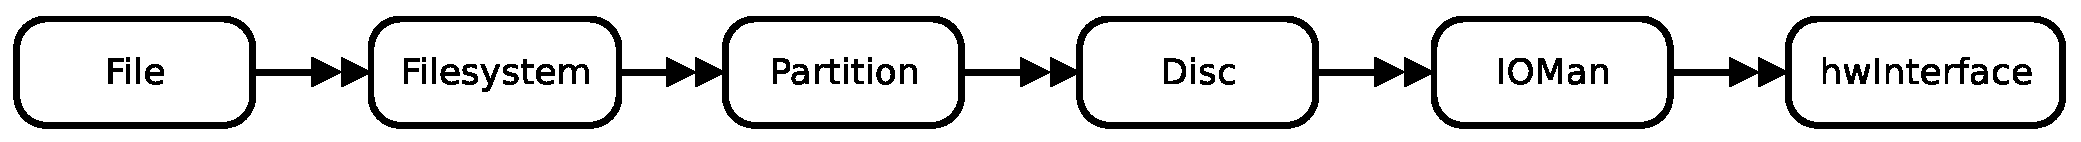
\includegraphics[scale=0.4]{schematics/objectmodel.eps}\\

As you can see we have created a linear object model that is quite simple.
The file en filesystem object deal with handling the filesystem specific stuff.
Below that we find the Partition object that is responsible for translating partition
relative addressing into disc-based LBA addressing.

The Disc object hold the partition table, and has a direct link to a cache manager, IOMan.
In IOMan, all requests for disc sectors come together. IOMan will perform checks to see
if sectors have to be read from disc (or from memory), or written back to disc.
In the latter case (reading or writing to disc), a request is made to the hardware layer.

The hardware interface has 3 responsibilities :
\begin{itemize}
	\item Initialize the hardware
	\item Read sectors from disc
	\item Write sectors to disc
\end{itemize}

All requests are \textsl{sector}based, a sector is a 512 byte piece from the disc, that is aligned to
a 512 byte boundary.\\\\
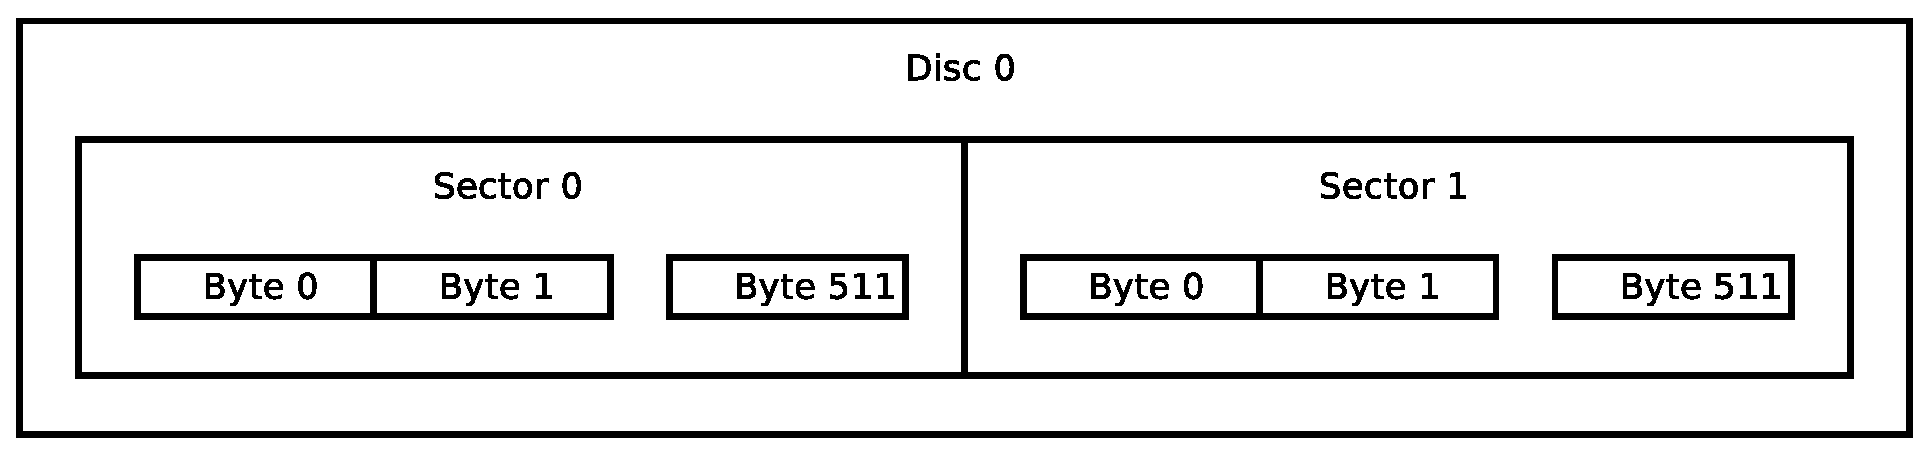
\includegraphics[scale=0.4]{schematics/sector.eps}

In this example we will create a new endpoint that will add support for data over pigeon carrier
for the EFSL. Initializing the hardware will require feeding the pigeon and telling it where the
data is. Reading/Writing will entail giving the bird the sector and letting it fly.

Perform the following steps:
\begin{enumerate}

	\item Choose a name for your endpoint\\
	You will need this name to create the required defines in the source code.
	For our example I've chosen the name \code{PIGEON\_CARRIER}.
	For consistency the final name is then \code{HW\_ENDPOINT\_PIGEON\_CARRIER}.

	\item Verify the sizes of integers\\
	Open \filename{inc/types.h} and create a new entry for pigeon carriers. Perhaps
	one of the existing sets is identical to yours and you can copy-paste it.

	\item Add your endpoint to \filename{interface.h}\\
	Locate the file \filename{interface.h} located in the directory \filename{inc/}
	Add a pigeon entry (located above the \code{\#else ... NO INTERFACE DEFINED})
\begin{lstlisting}
#if defined(HW_ENDPOINT_0)
   		#include "interfaces/0.h"
#elif defined(HW_ENDPOINT_1)
        #include "interfaces/1.h"
#elif defined(HW_ENDPOINT_PIGEON_CARRIER)
        #include "interfaces/pigeon.h"
#else
        #error "NO INTERFACE DEFINED - see interface.h"
#endif
\end{lstlisting}

	\item Select your endpoint in \filename{conf/config.h}
	
	\item Create your sourcefiles\\
	Create a header file in \filename{inc/} and a sourcefile in \filename {src/interfaces}.
	In this example I'm using \filename{pigeon.h} and \filename{pigeon.c}.

	\item Add your object file to the Makefile
	Take the Makefile that works best on your platform (they should all work with
	GNU/Make), or create a new one, using the existing one's as a template.
	Make sure to include your new pigeon object to the library.
	If you have an 'ar' like utility you can create a static library, else you may
	have to create a new project containing all required source files.

\end{enumerate}

The basic framework is now complete, now all that's left to do is to write the code
that will perform the actual flying work.

\subsubsection{hwInterface}
This structure represents the underlying hardware. There are some field that are required
to be present (because EFSL uses them), but you may put in as much or a little as
your driver requires to access the hardware.

As always in embedded design it is recommended to keep this structure as small
as possible.

Example:
\begin{lstlisting}
struct hwInterface{
	/* Field created for THIS hardware */
	Pigeon pigeon;

	/* Obligatory fields */
	euint32 sectorCount;
};
typedef struct hwInterface hwInterface;
\end{lstlisting}

\subsubsection{if\_initInterface}
This function will be called one time, when the hardware object is initialized 
by \code{efs\_init()}. This code should bring the hardware in a ready to use 
state.

The function's prototype is\\
\code{esint16 if\_initInterface(hwInterface *hw, euint8* opts);}

Optionally but recommended you should fill in the hw->sectorCount field with the number
of sectors. This field is used to validate sectorrequests.

An example of a initInterface function :
\begin{lstlisting}
esint16 if_initInterface(hwInterface *hw, euint8* opts)
{
	/* Parse options */
	parse_options(opts); /* Your application may not need options */

	/* Check hardware state */
	if(!alive(hw->pigeon)){
		//printf("Pigeon died! :-(\n");
		return(DEAD_PIGEON); /* #define DEAD_PIGEON -1 */
	}

	/* Initialize hardware */
	feed(hw->pigeon);
	pet (hw->pigeon);

	/* Get sectors count */
	hw->numSectors = ask_pigeon_num_sectors(hw->pigeon);

	return(0);
}
\end{lstlisting}

\subsubsection{if\_readBuf}
This function is responsible to read a sector from the disc and store it in a user supplied buffer. You will receive the hardware object, an address and a pointer to memory for storing
the buffer.

Please be very careful to respect the boundaries of the buffers, since it will usually be IOMan
calling this function, and if you have a buffer overflow you might corrupt the cache of the
the next buffer, which in turn may produce extremely rare and impossible to retrace behavior.

The function prototype is:\\
\code{esint16 if\_readBuf(hwInterface *hw,euint32 address, euint8* buf);}

The address is an LBA address, relative to the beginning of the disc. Should you be
accessing an old hard disc, or a device which uses some other form of addressing you will have to
recalculate the address to your own addressing scheme. Please note that there is no support
for sectors that are not 512 bytes large.

\begin{lstlisting}
esint8 if_readBuf(hwInterface* hw,euint32 address,euint8* buf)
{
	Message new_message;

	new_message.address = address;
	new_message.command = READ;

	pigeon_send(hw->pigeon,new_message); /* Launches the pigeon */
	while(!pigeon_returned(hw->pigeon)); /* Wait until the bird is back */
	memcpy(new_message.data,buf,512); /* Copy buffer */
	return(0);
}
\end{lstlisting}

\subsubsection{if\_writeBuf}
The function \code{if\_writeBuf} works exactly the same as it's reading variant.

\subsection{I/O Manager (0.2)}
	\label{ioman}
The IOManager that is the second lowest layer of the embedded filesystems library is
responsible for coordinating disk input and output, as well as managing a caching 
system. This documentation describes the second implementation of IOMan, which includes
features such as :
\begin{itemize}
	\item Delayed write
	\item Buffer reference statistics
	\item Buffer exportable to users
	\item Support for cached direct I/O as well as indirect I/O
	\item Can allocate memory itself (on the stack), or you can do it yourself (heap)
\end{itemize}

\subsubsection{General operation}
Because of the limited memory nature of most embedded devices for which this library is
intended several design decisions were made to minimize memory usage. Some of these required
that some concessions be made. One of them is that there is no memory protection, since
most devices don't have the memory to support this, or lack the ability to protect memory.

When IOMan receives a request for a sector, it will make sure it has the sector in it's
own memory cache and then give the caller a \code{euint8*} pointer to that cache. The
user is then free to do operations on that memory, and when it is done it should tell
IOMan so. Several things can go wrong with this: you can request a sector for reading,
and then write in the cache, thereby corrupting it. Or you can request a sector, but never
release it (sort of a memory leak), which may result in very bad performance, and a deadlocked
I/O manager.

But, taking into account that very little memory is required for operation, if you follow the I/O man rules, you will get a pretty clever caching object that will make writing new filesystems
a simple job.

\subsubsection{Cache decisions}
Whenever ioman receives a request to fetch a sector, be it read or write, it will have to make sure
it has, or can get the sector you want. It follows a certain path to do this.\label{cachemethod}
\begin{enumerate}
	\item First of all it will scan it's cache range to see if it already has the sector.
		If it is found, and it was a write request, the cache is marked writable. Usage and
		reference get incremented and a pointer	is then returned to the requester. If the
		buffer cannot be found, ioman proceeds to step 2.
	\item When an item is not in cache, it has to be fetched from the disc, the best place to
		store it is in memory that does not contain anything useful yet. Ioman will search for
		a place that is currently not occupied by anything. If it is found, the sector will be 
		placed on that spot and a pointer returned. Else, ioman proceeds to step 3.
	\item Since there is no other choice than to overwrite an already existing cache, ioman will
		try to find one that is the least interesting. First it will search for caches that
		are marked not writable, and have no users. Ioman will then select the one that has the
		least references. If there are none, it will search for caches that don't have users and
		are writable. Once again the one with the least references is returned. Since it is 
		writable ioman will flush it to disc first. After that the requested sector is put there
		and a pointer returned. If it cannot find any caches that have no users it will go to
		step 4.
	\item Since every cache spot is in use ioman will have to select one for overallocation.
		Since this selection depends on many factors and is rather complex, a points
		system is used. The algorithm considers every cache place and allocated a certain number
		of points to it, lower means that it is a better candidate for overallocation. Fifty 
		percent of the points goes to the cache being marked writable, since having to write
		a sector is expensive. Another 35 percent goes to how many overallocations have 
		already been done on that spot. It doesn't make sense to always overalloc the same buffer,
		it is better to spread this. The remaining 15 percent is determined by the number of 
		references to the sector. 
		
		After a function has selected the best candidate, ioman will overwrite that spot with
		the new sector. It will also push the status and sectornumber onto that cache's 
		retrieval stack, so that when the sector is released, the older sector can be retrieved.
		If this fails go to step 5.
	\item When ioman gets here it will return a (nil) pointer and flag an error.
\end{enumerate}

\subsubsection{Functions}

\begin{longtable}{|p{0.35\textwidth}|p{0.65\textwidth}|}
	
	\hline
	\multicolumn{2}{|c|}{
		\textbf{I/O Manager Functions}
	} \\
	\multicolumn{2}{|c|}{} \\
	\hline
	\hline
	\endfirsthead
	
	\hline
	\multicolumn{2}{|c|}{\textbf{I/O Manager Functions (continued)}} \\
	\hline
	\endhead

	\hline
	\endfoot
	
	\hline 
	\endlastfoot

	\code{ioman\_init} & \code{esint8 (IOManager *ioman, hwInterface *iface, euint8* bufferarea)} \\
	\hline
	\multicolumn{2}{|p{\textwidth}|}{
		This function is called to initialize the internal state of the I/O manager. It should be the
		first function you call on an ioman object. Failure to do so will result in undefined behavior.
		The function clears all internal variables to a default safe state, and sets up it's memory region.
		
		There are two possibilities, if you supply a 0 pointer then a function will be called that contains
		a static variable with a size of 512 * \code{IOMAN\_NUMBUFFERS}, else, it will be assumed that
		you allocated that memory yourself and the pointer you provided will be used.
	}\\
	\hline

	\code{\external{ioman\_reset}} & \code{void (IOManager *ioman)} \\
	\hline
	\multicolumn{2}{|p{\textwidth}|}{
		This function is called from the initialization function, it does the actual reset of all variables.
	}\\
	\hline

	\code{ioman\_pop} & \code{esint8 (IOManager *ioman,euint16 bufplace)} \\
	\hline
	\multicolumn{2}{|p{\textwidth}|}{
		This function fetches settings (sector number, usage and status register) from stack \code{bufplace}
		and puts it back on the main registers. It will return 0 on successful pop, and -1 on error, or when
		there are no elements to pop.
	}\\
	\hline

	\code{ioman\_push} & \code{esint8 (IOManager *ioman,euint16 bufplace)} \\
	\hline
	\multicolumn{2}{|p{\textwidth}|}{
		This function pushes the settings of cache \code{bufplace} onto that cache's stack. It does not 
		destroy the data in the main registers. It will return 0 for a successful push, and -1 on error, or
		when there is no more space to push a new element.
	}\\
	\hline

	\code{ioman\_readSector} & \code{esint8 (IOManager *ioman,euint32 address,euint8* buf)} \\
	\hline
	\multicolumn{2}{|p{\textwidth}|}{
		This function does the actual reading from the hardware, it is the one and only function that
		calls \code{if\_readBuf()}, here a retry on failure policy could be implemented. This function
		will correctly stream errors upwards. All calls made to this function in the iomanager are checked
		for their return value, so errors propagate correctly upwards. 
		
		The address it receives is relative to the beginning of the disc, no assumptions about \code{buf}
		may be made, it can be withing ioman's cache memory range, but it could also be a buffer from userspace.
		
		The function will return 0 on success and -1 on failure.
	}\\
	\hline

	\code{ioman\_writeSector} & \code{esint8 (IOManager *ioman, euint32 address, euint8* buf)} \\
	\hline
	\multicolumn{2}{|p{\textwidth}|}{
		This function does the actual writing to the hardware, it is the one and only function that
		calls \code{if\_writeBuf()}, here a retry on failure policy could be implemented. This function
		will correctly stream errors upwards. All calls made to this function in the iomanager are checked
		for their return value, so errors propagate correctly upwards. 
		
		The address it receives is relative to the beginning of the disc, no assumptions about \code{buf}
		may be made, it can be withing ioman's cache memory range, but it could also be a buffer from userspace.
		
		The function will return 0 on success and -1 on failure.
	}\\
	\hline

	\code{\external{ioman\_getSector}} & \code{euint8* (IOManager *ioman,euint32 address, euint8 mode)} \\
	\hline
	\multicolumn{2}{|p{\textwidth}|}{
		This function is the one that is called most from the higher library routines. It is the function
		that will present you with a pointer to memory containing sector number \code{address}. There are
		several modes that you can select or combine.\newline
		\begin{tabular}{|l|p{.6\textwidth}|}
		\hline
		\code{IOM\_MODE\_READONLY} & This attribute says to ioman that it needs a buffer only for reading.
		This does not mean that you are allowed to write to it, doing so results in undefined behavior.
		You cannot combine this option with the \code{IOM\_MODE\_READWRITE} option.\\
		\code{IOM\_MODE\_READWRITE} & This attribute says to ioman that it would like not only to read from
		but also to write to that buffer. When you release the sector your changes will be written to disc.
		This may not happen immediately though, if you want to force it take a look at the 
		\code{ioman\_flushRange()} function. This option cannot be combined with the 
		\code{IOM\_MODE\_READONLY} option.\\
		\code{IOM\_MODE\_EXP\_REQ} & This option tell the iomanager that the request is exceptional, for
		example that the request is unlikely to happen again. The library adds this flags to the options
		when requesting the bootrecord, to prevent it from getting a high rating, which should prevent it
		from being removed from the cache.\\
		\hline
		\end{tabular}\newline
		These options can be combined by ORing them together.
	}\\
	\hline

	\code{ioman\_releaseSector} & \code{esint8 (IOManager *ioman,euint8* buf)} \\
	\hline
	\multicolumn{2}{|p{\textwidth}|}{
		This function tells ioman that you are done with one of the cache elements and that it can do
		it's bidding with it. Forgetting to call this function may result in deadlocked iomanagers.
	}\\
	\hline

	\code{ioman\_directSectorRead} & \code{esint8 (IOManager *ioman,euint32 address, euint8* buf)} \\
	\hline
	\multicolumn{2}{|p{\textwidth}|}{
		This is a variant of the normal getsector. Sometimes you need a sector from the disc, but all
		you want to do with it is export it directly to userbuffers. It would be foolish to force a
		caching of that sector if there is external space available for it.
		
		This function will fetch sector \code{address} from disc and place it in the memory pointed to
		by \code{buf}. Should there be a free spot available the sector will be cached there, so that
		it may be used in the future. If the sector was available from cache in the first place, it
		will simply be \code{memCpy()}'d from the cache to the userspace buffer.
	}\\
	\hline

	\code{ioman\_directSectorWrite} & \code{esint8 (IOManager *ioman,euint32 address, euint8* buf)} \\
	\hline
	\multicolumn{2}{|p{\textwidth}|}{
		This function is based on the same philosophy as \code{ioman\_directSectorRead()}, however,
		contrary to what the name may lead to believe it also passes through a caching layer. If
		there is an unused spot (or the sector is in cache), the userbuffer will be copied to that
		spot and will remain there until the space is needed or a flush is forced.
	}\\
	\hline

	\code{ioman\_flushRange} & \code{esint8 (IOManager *ioman,euint32 address\_low, euint32 address\_high)} \\
	\hline
	\multicolumn{2}{|p{\textwidth}|}{
		This function is used to ask ioman to flush all sectors to disc that are in a specific
		range. For example you might want to flush a specific range of your filesystem without
		needlessly disturb other parts. The range is \code{address\_low <= n => address\_high}.
		Off course only sectors that are marked as writable are flushed to disc.
	}\\
	\hline

	\code{ioman\_flushAll} & \code{esint8 (IOManager *ioman)} \\
	\hline
	\multicolumn{2}{|p{\textwidth}|}{
	This function will cause ioman to flush out all cache units that are marked writable. If
	they do not have any users, they will lose their writable mark.
	}\\
	\hline
\end{longtable}


\subsection{C library for EFSL (0.2)}
	This section of the manual describes the minimalistic C library functions that were
created for EFSL. Since EFSL was designed for ultimate portability, no assumptions about the
workings or even the presence of a C library could be made. Fortunately only very few functions
had to be created that mimicked the operations of well known C library functions.
\\
\begin{longtable}{|p{0.35\textwidth}|p{0.65\textwidth}|}
	
	\hline
	\multicolumn{2}{|c|}{
		\textbf{PLibC Functions}
	} \\
	\multicolumn{2}{|c|}{} \\
	\hline
	\hline
	\endfirsthead
	
	\hline
	\multicolumn{2}{|c|}{\textbf{PLibC Functions (continued)}} \\
	\hline
	\endhead

	\hline
	\endfoot
	
	\hline 
	\endlastfoot

	\code{strMatch} & \code{euint16 strMatch(eint8* bufa, eint8*bufb,euint32 n)} \\
	\hline
	\multicolumn{2}{|p{\textwidth}|}{
	This function compares the strings \code{bufa} and \code{bufb} for \code{n} bytes.
	It will return the number of bytes in that section that does not match. So if you
	want to compare two strings the return value should be 0, for the strings to match over
	the entire \code{n} area.
	}\\
	\hline
	
	\code{memCpy} & \code{void memCpy(void* psrc, void* pdest, euint32 size)} \\
	\hline
	\multicolumn{2}{|p{\textwidth}|}{
	This function will copy the contents at location \code{psrc} to location \code{pdest} over
	a range of \code{size} bytes.
	}\\
	\hline

	\code{memClr} & \code{void memClr(void *pdest,euint32 size)} \\
	\hline
	\multicolumn{2}{|p{\textwidth}|}{
	This function will set the memory at \code{pdest} to value \code{0x00} for a range of
	\code{size} bytes.
	}\\
	\hline

	\code{memSet} & \code{void memSet(void *pdest,euint32 size,euint8 data)} \\
	\hline
	\multicolumn{2}{|p{\textwidth}|}{
	This function will set the memory at \code{pdest} to value \code{data} for a range of
	\code{size} bytes.
	}\\
	\hline
\end{longtable}


	
\newpage
\section{Legal notes}
	This library is subject to the Lesser General Public License version 2.1.
We have chosen this license in stead of the BSD license because we feel strongly
that more effort was needed in the field of quality software in the embedded field.

Please note that if you make changes to the library itself, those modifications must be
made public, but that writing support for new hardware and linking it into the library,
does not fall under this category. However, we would off course appreciate it tremendously
if you would send us in code to support new hardware.

\subsection{GNU Lesser General Public License}
\verbatiminput{pages/lgpl.txt}



\end{document}
